\chapter{Astroteilchenphysik}
\label{chapter:Astroteilchenphysik}
Die Astroteilchenphysik ist ein noch recht junger Teilbereich der Physik und beinhaltet Fragen der Astrophysik und der Teilchenphysik.
Verschiedene Botenteilchen, deren Eigenschaften in \autoref{sec:KosmischeStrahlung} beschrieben werden, geben Auskünfte über astrophysikalische Quellen, welche in \autoref{sec:Quellen} erklärt werden.
Diese Quellen emittieren geladene, bzw.  ungeladene Teilchen, die mit Hilfe von Satelliten im All oder auf der Erde detektiert werden.
%Die Energie dieser in den Quellen beschleunigten Teilchen übersteigt zum Teil die höchste Energie, die auf der Erde mit Beschleunigern erreicht werden kann.
Die Modelle für die grundlegenden Beschleunigungsmechanismen der Teilchen, die in \autoref{sec:Beschleunigungsmechanismen} beschrieben werden, müssen noch überprüft bzw. weiterentwickelt werden.
Im Laufe der Jahre wurden verschiedene Detektionsmethoden entwickelt, die speziell an die zu detektierenden Teilchen angepasst sind.
Gleichwohl ist die Forschung in der Detektorentwicklung noch nicht abgeschlossen und die Kollaborationen, sowie die konzipierten Detektoren werden fortschrittlicher und damit verbunden auch oft größer.
Beispiele dafür sind der IceCube-Neutrino-Detektor oder das geplante Cherenkov-Teleskop-Array CTA.
\autoref{sec:Gammaastronomie} bietet eine Übersicht über die Gammaastronomie und beschreibt die Wechselwirkung der Photonen auf dem Weg von der Quelle zum Detektor. 
Im \autoref{sec:AGN} wird noch einmal der spezielle Quelltyp des Aktiven Galaktischen Kerns (AGN: Active Galctic Nuclei) näher beschrieben.
\autoref{sec:Mrk421} bietet eine Übersicht über die Quelle Mrk 421, die im Verlauf dieser Arbeit näher untersucht wird.

\section{Kosmische Strahlung}
\label{sec:KosmischeStrahlung}

\begin{figure}
    \centering
    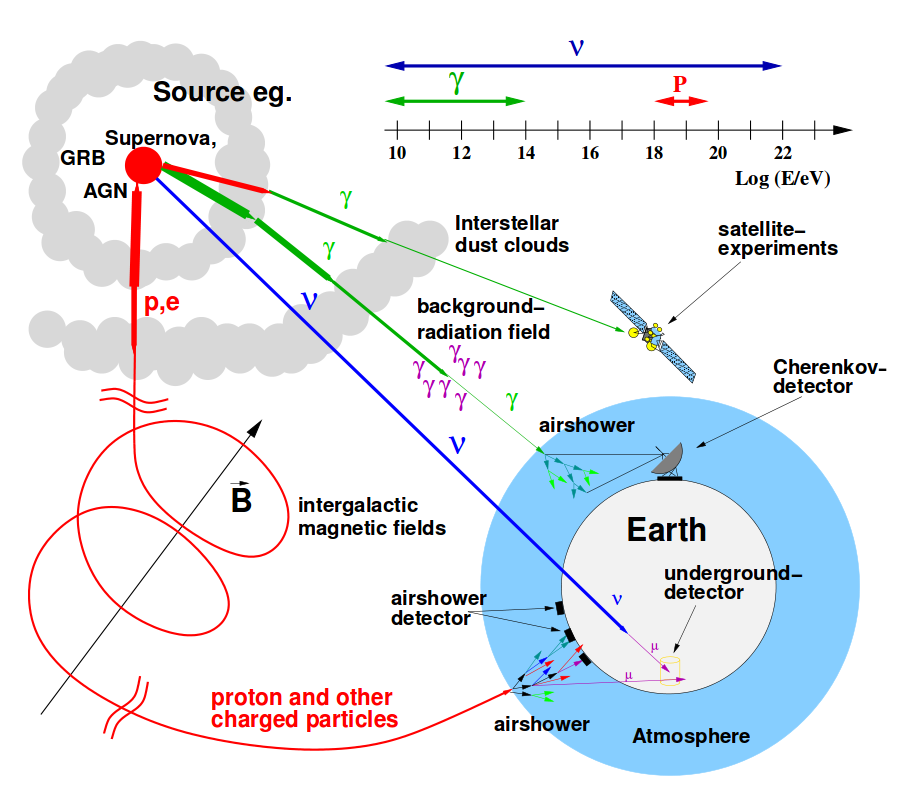
\includegraphics[width=0.8\textwidth]{./Plots/02_Astroteilchenphysik/Astroteilchen.png}
    \caption{Schematische Darstellung der Wechselwirkungen, sowie der Detektion der Botenteilchen auf dem Weg von der Quelle zum Beobachter.
    Auf ihrem Weg unterliegen die unterschiedlichen Botenteilchen unterschiedlichen Wechselwirkungen. 
    Geladene Teilchen wechselwirken mit Staubwolken und werden von Magnetfeldern abgelenkt, Neutrinos und hochenergetische Photonen behalten ihre Richtungsinformation bei.
    Photonen wechselwirken ebenfalls mit Staubwolken oder mit niederenergetischen Hintergrundphotonen und werden dann abhängig von ihrer Energie mit unterschiedlichen Detektoren gemessen. 
    Das Bild entstammt \cite{DissMarlene}.}
    \label{Astroteilchen}
\end{figure}


\autoref{Astroteilchen} zeigt eine schematische Darstellung verschiedener Botenteilchen, die von einer astrophysikalischen Quelle emittiert werden können.

In \autoref{Astroteilchen} werden schematisch die Eigenschaften der Botenteilchen auf ihrem Weg von der Quelle zum Beobachter dargestellt.
Geladene Teilchen wie Protonen oder Elektronen wechselwirken im Allgemeinen mit intergalaktischen oder interstellaren Magnetfeldern.
Dadurch stellt die Rekonstruktion ihrer Ursprungsrichtung eine Herausforderung dar.
Im Gegensatz zu den geladenen Teilchen, können Neutrinos aufgrund ihrer geringen Wechselwirkungswahrscheinlichkeit diese Strecke nahezu ungehindert zurücklegen. 
Allerdings ist ihre Detektion schwierig, sodass nur Detektoren mit sehr großem Volumen sie indirekt über ihre Sekundärteilchen detektieren können.
Diese Detektion geschieht z.B. mit IceCube, einem Detektor, der in das Eis am Südpol eingeschmolzen, folgendermaßen:
Ein Neutrino wechselwirkt mit einem Nukleon und erzeugt dabei ein geladenes Lepton. 
Beim Durchgang durch den Detektor produziert dieses geladene Lepton Cherenkov-Strahlung, die mit Hilfe von Photosensoren detektiert wird.
Photonen besitzen den gleichen Vorteil wie Neutrinos und werden auf dem Weg zum Detektor nicht abgelenkt.
Allerdings können sie direkt mit Staubwolken oder der niederenergetischen Hintergrundstrahlung (EBL: External Background Light), welche aus Sternenlicht oder Wärmestrahlung aus interstellarem Staub besteht, wechselwirken.
Hochenergetische Photonen werden von Satellitenexperimenten oder von Luftschauerteleskopen detektiert.
Die Detektion mit Satellitenexperimenten geschieht direkt, während Luftschauerteleskope die Teilchen indirekt detektieren.
Wie in \autoref{sec:Gammaastronomie} beschrieben wird, werden die Luftschauer vermessen und daraus auf die Eigenschaften des Primärteilchens geschlossen.


\subsection{Die geladene kosmische Strahlung}
Die geladene kosmische Strahlung wurde Anfang des 20. Jahrhunderts mit Hilfe von Ballonexperimenten entdeckt \cite{Hess}.
Aufgrund des Ergebnisses, dass mit steigender Höhe die Ionisation zunahm, schlossen Hess und Kohlhörster \cite{Kohlhoerster}, dass die von ihnen detektierte Strahlung aus dem Weltraum kommt.
Diese Strahlung besteht zu 85\% aus Protonen, zu 12\% aus $\alpha$-Teilchen und 3\% aus Elementen mit größerer Kernladung \cite{Grupen}.
Das Energiespektrum dieser kosmischen Strahlung ist auf einem sehr großen Energiebereich vermessen und wurde sowohl mit erdgebundenen Experimenten als auch mit Satellitenexperimenten bestimmt.


\begin{figure}
    \centering
    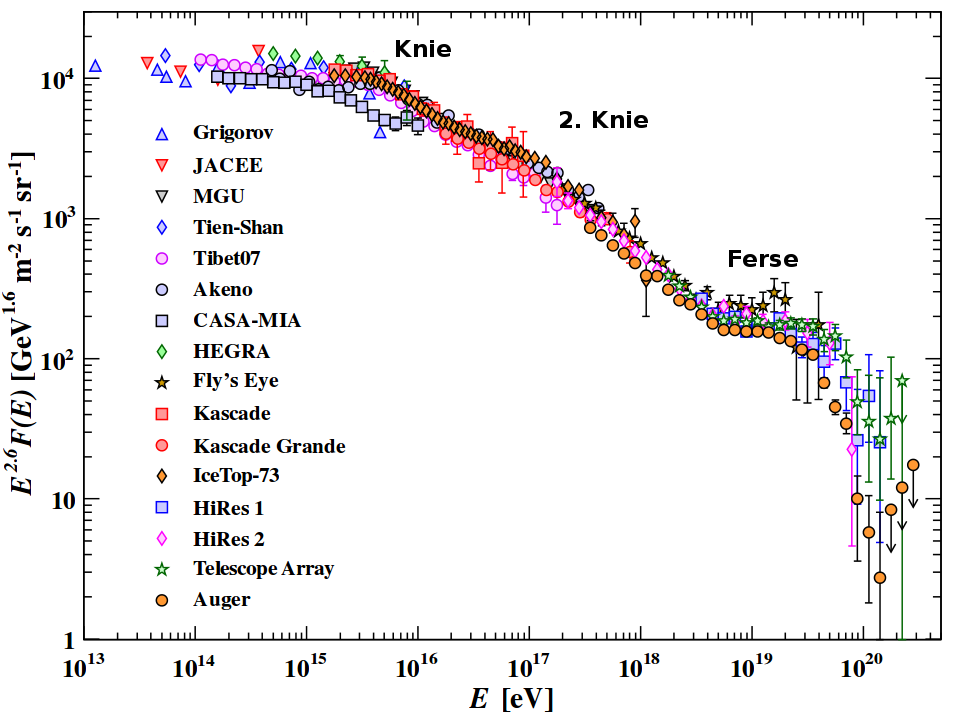
\includegraphics[width=0.9\textwidth]{./Plots/02_Astroteilchenphysik/CosmicRaySpectrum2.png}
    \caption{Spektrum der kosmischen Strahlung. 
      Aufgetragen ist der mit $E^{2,6}$ gewichtete Fluss der Teilchen gegen die Primärteilchenenergie. 
      Bei der Energie $E=10^{6,4}\,\si{GeV}$ befindet sich das sogenannte "Knie" und bei der Energie $E=10^{9,5}\,\si{GeV}$ die "Ferse" des Spektrums. 
      Bei der Energie $E=4\cdot 10^8\,\si{GeV}$ \cite{Knie} wird das zweite Knie erwartet.\cite{PDG}}
    \label{CR-Spektrum}
\end{figure}



Wie in \autoref{CR-Spektrum} zu erkennen ist, kann das Spektrum mit einem gebrochenen Potenzgesetz mit zwei Steigungsänderungen, die als "Knie" und "Ferse" bezeichnet werden, parametrisiert werden \cite{Knie}.
Hierbei ist $N$ die Anzahl, $E$ die Energie, $E_p$ die Primärteilchenenergie und $\alpha_{CR}$ der spektrale Index der kosmischen Strahlung:

\begin{equation}
 \frac{\mathrm{d}N}{\mathrm{d}E} \propto E_p^{-\alpha_{CR}}
\end{equation}

mit \cite{Knie} 

\begin{equation*}
\alpha_{CR}=	
\left\{
\begin{aligned}
2,7 \qquad &E   \leq \SI{4,5e6}{GeV} \\
3,10 \qquad &  \SI{4,5e6}{GeV} < E  \leq \SI{4e9}{GeV} \\ 
2,7 \qquad & E > \SI{4e9}{GeV}.
\end{aligned}
\right.
\end{equation*}

Die Existenz eines zweiten Knies bei $E=4\cdot 10^8\,\si{GeV}$\cite{Knie} wird noch untersucht.

Größere Energien als $\SI{5e19}{eV}$ können aufgrund des GZK-Cutoffs \cite{Greisen}\cite{ZatsepinKuzmin} nur schwer gemessen werden, da sie auf großen Propagationslängen stark unterdrückt sind . 
Dieser Cutoff tritt auf, wenn Protonen mit dem kosmischen Mikrowellenhintergrund (CMB) wechselwirken \cite{Greisen}\cite{ZatsepinKuzmin}: 

\begin{equation*}
p\gamma_{CMB}=	
\left\{
\begin{aligned}
& \Delta^+ \\
& p\, e^+ \, e^- .
\end{aligned}
\right.
\end{equation*}

Knie und Ferse beinhalten Informationen über die Beschleunigungsmechanismen der Teilchen bzw. über die Quellen.
Die Teilchen mit den höchsten Energien jenseits der Ferse können nicht galaktischen Ursprungs sein, da die galaktischen Magnetfelder für die Beschleunigung zu schwach sind. 
Deswegen wird vermutet, dass diese Teilchen extragalaktischen Ursprungs sind, wobei die Beschleunigungsmechanismen (vgl. \autoref{sec:Beschleunigungsmechanismen}) noch nicht genau bekannt sind.

\subsection{Neutrinos als Botenteilchen}
Neutrinos sind leichte Teilchen, die eine sehr geringe Wechselwirkungswahrscheinlichkeit aufweisen und daher nur in großen Experimenten wie IceCube \cite{Icecube} oder ANTARES \cite{ANTARES} indirekt über ihre leptonischen Partner nachgewiesen werden können.
Es gibt verschiedene Quellen, in denen Neutrinos entstehen können.
Kosmogene Neutrinos werden in Wechselwirkungen von hochenergetischen Protonen mit dem kosmischen Mikrowellenhintergrund (CMB: Cosmic Miocrowave Background) und dem darauffolgenden Zerfall von geladenen Pionen erzeugt.
Galaktische Neutrinos können in hadronischen Beschleunigungsprozessen erzeugt werden.
Es wird auch vermutet, dass in Gammastrahlenausbrüchen oder in hadronischen Beschleunigungsprozessen in AGNs Neutrinos entstehen können.

Die größte Herausforderung bei der Suche nach hochenergetischen Neutrinos ist der Untergrund, der durch Wechselwirkungen von geladener kosmischer Strahlung mit der Atmosphäre entsteht.
% Neutrinos werden in hadronischen Reaktionen erzeugt und können auf dem Weg von der Quelle zum Detektor oszillieren.
Die Produktion von Neutrinos geschieht über schwache Zerfälle von Hadronen, hauptsächlich Pionen.
Nachfolgend werden die möglichen Reaktionen beschrieben.
Entweder wechselwirkt ein Photon mit einem Proton (mit der in Klammern angegebenen Wahrscheinlichkeit) \cite{DissBecker}:

\begin{equation*}
p\, \gamma \rightarrow \Delta^+ \, \rightarrow	
\left\{
\begin{aligned}
& p \, \pi^0 & \qquad (2/3) \\
& n \, \pi^+ & \qquad (1/3)
\end{aligned}
\right.
\end{equation*}.

Oder ein Proton wechselwirkt mit einem anderen Proton \cite{DissBecker}:

\begin{equation*}
p \, p \rightarrow
\left\{
\begin{aligned}
& p \, p \, \pi^0 & \qquad (2/3) \\
& p \, n \, \pi^+ & \qquad (1/3).
\end{aligned}
\right.
\end{equation*}

Bei höheren Energien tragen auch Kaonen und Neutronen zur Neutrinoproduktion bei.
In diesen Prozessen entstehen negativ geladene Pionen, die zerfallen und dabei Neutrinos produzieren \cite{NeutrinoOszillation}.
% Die gleichen Prozesse treten auch für Neutronen oder bei höheren Energien Kaonen als Primärteilchen auf, wodurch negativ geladene Pionen entstehen.
% Die Pionen zerfallen dann und erzeugen weitere Neutrinos \cite{DissBecker}:

\begin{equation*}
 \begin{aligned}
 \pi^+ \rightarrow \mu^+ \, \nu_{\mu} \rightarrow e^+ \, \nu_e \, \overline{\nu}_{\mu} \, \nu_{\mu} \\ 
 \pi^- \rightarrow \mu^- \, \overline{\nu}_{\mu} \rightarrow e^- \, \overline{\nu}_e \, \nu_{\mu} \, \overline{\nu}_{\mu}
 \end{aligned}
\end{equation*}


In der Quelle wird eine Verteilung der Neutrinos von $(\nu_e:\nu_{\mu}:\nu_{\tau})=(\overline{\nu}_e:\overline{\nu}_{\mu}:\overline{\nu}_{\tau})=(1:2:0)$ erwartet \cite{NeutrinoOszillation}.
Aufgrund von Neutrinooszillationen wird auf der Erde ein Verhältnis von $(\nu_e:\nu_{\mu}:\nu_{\tau})=(1:1:1)$ \cite{NeutrinoOszillation} beobachtet.

%Aufgrund der beschriebenen Prozesse erwartet man in der Quelle eine Verteilung der Neutrinos von $(\nu_e:\nu_{\mu}:\nu_{\tau})=(\overline{\nu}_e:\overline{\nu}_{\mu}:\overline{\nu}_{\tau})=(1:2:0)$.
%Propagieren die Neutrinos Strecken von der Größenordnung des Sonnensystems, oszillieren sie, sodass auf der Erde ein Verhältnis von $(\nu_e:\nu_{\mu}:\nu_{\tau})=(1:1:1)$ beobachtet wird.


\subsection{Photonen als Botenteilchen}
\label{subsec:Photonen}
Genau wie die Neutrinos besitzen Photonen den Vorteil, dass sie nicht von Magnetfeldern abgelenkt werden.
Allerdings können aufgrund der Absorption in der Atmosphäre auf der Erde nur Photonen im optischen und im Radiobereich direkt detektiert werden.
Deswegen hat sich die optische Astronomie und die Radioastronomie zuerst entwickelt. 
%Deswegen wurden diese Wellenlängen in der Astronomie auch als erstes benutzt. 
Danach kamen dann Astronomie mit anderen Wellenlängen wie Röntgenstrahlung oder Gammastrahlung hinzu.
Gammastrahlung lässt sich anhand der Energie in nieder- bis mittelenergetische Gammastrahlung ($\SI{0,1}{MeV}$ - $\SI{30}{MeV}$), hochenergetische Gammastrahlung ($\SI{30}{MeV}$ -$\SI{100}{GeV}$), sehr hochenergetische Gammastrahlung ($\SI{100}{GeV}$-$\SI{100}{TeV}$) und ultrahochenergetische Gammastrahlung ($E>\SI{100}{TeV}$) einteilen.

% Der Energiebereich bis ca. 100GeV lässt sich nur mit Satellitenexperimente nachweisen.
% Die sehr hochenergetische und die ultrahochenergetische Strahlung lässt sich wiederum mit Hilfe von Luftschauerteleskopen auf der Erde detektieren.\cite{Weekes}

Der Nachteil der hochenergetischen Photonen ist, dass sie mit den niederenergetischen Photonen der Hintergrundstrahlung (EBL) wechselwirken.
Mit Hilfe von Messungen können dann Modelle erstellt werden, die die Hintergrundstrahlung parametrisieren und mit Hilfe derer dann diese Absorption in Beobachtungen berücksichtigt werden kann.

%Mit Hilfe von Modellen kann die Absorption von hochenergetischen Photonen aus extragalaktischen Quellen durch diese Hintergrundstrahlung berechnet werden.\cite{Weekes}

\autoref{sec:Gammaastronomie} geht näher auf die Gammaastronomie ein und es werden die Wechselwirkungen erklärt, die die Photonen auf ihrem Weg zur Erde erfahren.


\section{Quellen kosmischer Strahlung}
\label{sec:Quellen}
In diesem Kapitel wird eine Übersicht über einige Quellen der kosmischen Strahlung gegeben.
Es werden vor allem die wichtigsten Quellen hochenergetischer Gammastrahlung vorgestellt.

\subsection{Die Galaktische Scheibe und das Galaktische Zentrum}
1968 wurde das erste Mal Gammastrahlung von der Galaktischen Scheibe detektiert \cite{GalacticPlane}.
Diese galaktische Gammastrahlung kann in verschiedenen Prozessen entstehen, die Photonen unterschiedlicher Energien erzeugen.
Niederenergetische Photonen können durch Bremsstrahlung von Elektronen im interstellaren Gas erzeugt werden.
Elektronen können auch in einem inversen Comptonprozess an niederenergetischen Photonen gestreut werden, wodurch die Photonen auf hohe Energien beschleunigt werden.
Im Zerfall von neutralen Pionen zu Photonen werden Photonen mittlerer Energie erzeugt.



%Die galaktische Scheibe ist die stärkste und erste detektierte Gammaquelle und wurde 1968\cite{GalacticPlane} detektiert.
%Im Folgenden werden die Prozesse beschrieben, die die galaktische Gammastrahlung erzeugen:

% \begin{itemize}
%  \item Kosmische Elektronen erzeugen niederenergetische Photonen durch Bremsstrahlung mit dem Interstellaren Gas.
%  \item Hadronen der kosmischen Strahlung produzieren neutrale Pionen, die dann in zwei Photonen mit mittlerer Energie zerfallen.
%  \item Kosmische Elektronen überleben eine inverse Comptonstreuung an niederenergetischen Gammaphotonen und erzeugen Photonen mit hohen Energien.
% \end{itemize}

Das Galaktische Zentrum enthält mehrere massive Objekte, wie junge Supernova-Überreste, die hochenergetische Gammastrahlen emittieren.
So befindet sich in einem Radius von $\SI{10}{pc}$ um das Galaktische Zentrum eine Masse von $3\cdot 10^7$ Sonnenmassen. 
%Das dynamische Zentrum wurde mit der kompakten Radioquelle Sgr $A^*$ assoziiert, welche vermutlich ein supermassives schwarzes Loch ist.
Dem Satellitenexperiment EGRET gelang die Detektion einer Quelle - 3EG J1745-2852 - von hochenergetischer Gammastrahlung.
Allerdings ist die Natur dieser Quelle noch unbekannt.\cite{GalacticCenter}\cite{Weekes}



% In einem Radius von $\SI{10}{pc}$ um das Galaktische Zentrum befindet sich eine Masse von $3\cdot 10^7$ Sonnenmassen.
% Das Satellitenexperiment EGRET hat die Quelle 3EG J1745-2852 detektiert, welche hochenergetische Gammastrahlung emittiert. 
% Die Natur dieser Quelle ist noch unbekannt.\cite{GalacticCenter}\cite{Weekes}


\subsection{Supernovae und Supernovaüberreste}
Die Explosion eines Sterns wird als Supernova (SN) bezeichnet.
Gammastrahlung, die aus einer SN kommt, wird entweder in den ersten Sekunden der Explosion als Gammastrahlungsausbruch (GRB: Gamma Ray Burst) emittiert.
Falls nach dem GRB ein Pulsar entsteht, kann sie aber auch auch als stete periodische Emission dieses Pulsars abgestrahltt werden.
Es ist auch möglich, dass die Photonen aus der sich ausbreitenden Hülle des ehemaligen Sterns (SNR: Supernova Remnant) stammen. 
Diese galaktischen Quellen liefern kosmische Strahlung bis zu Energien von $\SI{100}{TeV}$ \cite{Weekes}.
Eine Beschleunigung von Teilchen auf Energien von $10^{20}\,\si{eV}$ durch SN und SNR ist nicht möglich.
Teilchen mit so hohen Energien stammen somit aus extragalaktischen Quellen.\cite{Weekes}

% Die Beschleunigung der Teilchen erfolgt in Schockwellen.
% Das Modell dieser diffusen Schockbeschleunigung liefert ein Potenzgesetz für das Spektrum der beschleunigten Strahlung von $\frac{dN}{dE} \propto E^{-2,0}$.
% Dieses Potenzgesetz wird um Effekte während der Propagation durch die Galaxie korrigiert und resultiert in einem Spektrum der kosmischen Strahlung von $\frac{dN}{dE} \propto E^{-2,7}$
% Im Allgemeinen sind die Spektra von Supernovae hart und haben einen Cutoff bei ca. $\SI{20}{TeV}$, was auf eine Primärteilchenenergie von einigen TeV schließen lässt.\cite{Weekes}\cite{RhodeFalke}


\subsection{Pulsare und Binäre Systeme}
Pulsare sind rotierende Neutronensterne mit einer Rotationsperiode zwischen einigen Millisekunden und einigen Sekunden.
Das bekannteste Beispiel ist der Crab-Pulsar im Zentrum des Krebsnebels.

Dieser Quelltyp wurde vor mehr als 30 Jahren entdeckt und lässt sich in zwei Kategorien einteilen.
Pulsare der ersten Kategorie gewinnen ihre Energie durch Rotation und sind im Allgemeinen im Radiobereich gut detektierbar.
Pulsare der zweiten Kategorie gewinnen ihre Energie durch Akkretion von Materie und sind vor allem im Röntgenbereich sichtbar.
Die Emissionsprozesse der Pulsare der zweiten Kategorie sind rein thermisch und von weniger Interesse für die hochenergetische Gammaastronomie.

Bisher wurden einige Pulsare entdeckt, die im Gammabereich ebenfalls eine hohe Luminosität haben.
Genau wie bei SNe und SNRs, können ihre Energiespektren durch ein Potenzgesetz beschrieben werden.
Verschiedene Pulsare lassen sich anhand ihrer Spektren voneinander unterschieden.
Ihre Lichtkurven unterscheiden sich in der Position der Peaks bei verschiedenen Wellenlängen.
Die Emissionsmechanismen von Pulsaren sind noch nicht komplett verstanden und zwei Modelle konkurrieren miteinander.
Eine detaillierte Beschreibung dieser Modelle kann \cite{Weekes} entnommen werden.

Die Hälfte aller Sterne taucht in einer Assoziation mit einem anderen Objekt auf und wird Binäres System genannt.
Dieses andere Objekt ist oft ein kompaktes Objekt wie ein Weißer Zwerg, ein Neutronenstern oder ein Schwarzes Loch.
Hohe Röntgenemission sowie ein zeitlich variables Verhalten sind charakteristisch für diesen Quelltyp.
Die Variabilität kann im Bereich von Millisekunden bis zu Jahren liegen und periodisch auftauchen oder in einzelnen Ausbrüchen wird viel Strahlung emittiert.\cite{Weekes}


\subsection{Gammastrahlenausbrüche}
Gammastrahlenausbrüche (GRB: Gamma Ray Burst) wurden während des kalten Kriegs von den amerikanischen \textit{Vela}-Satelliten, die Atombombenexplosionen aufspüren sollten, entdeckt.
16 GRBs mit Zeitspannen von $\SI{0,1}{s}$ - $\SI{30}{s}$ und Teilchenflüssen zwischen $(10^{-5}-10^{-4}\,\frac{\si{erg}}{\si{s}}$ wurden detektiert.

Im Allgemeinen dauern GRBs zwischen Millisekunden und einigen tausend Sekunden an und sind isotrop verteilt.
Sie werden in kurzweilige Ausbrüche ($t<\SI{2}{s}$) und den Rest unterteilt.
Fast die gesamte emittierte Energie ist größer als $\SI{50}{keV}$.
Mit Satellitenexperimenten wurden GRBs auch bei Energien von Gammastrahlung (bis ca. $\SI{30}{GeV}$) detektiert, der Fluss, d.h. die Anzahl der Teilchen pro Fläche und Zeit, ist aber sehr niedrig.
Bodengebundene Teleskope, z.B. MAGIC, betreiben GRB-Programme, allerdings kam es bisher noch zu keiner Detektion.\cite{Weekes}


\subsection{Aktive Galaktische Kerne}
Die Klasse der Aktiven Galaktischen Kerne (AGN) wird durch ein supermassives Schwarzes Loch, welches sich in ihrem Zentrum befindet und Materie akkretiert, gekennzeichnet.
Abhängig vom AGN-Typ werden aus dem Zentrum noch zwei Jets in entgegengesetzte Richtungen emittiert.  
Anhand ihrer Ausrichtung zum Beobachter und ihrer Emission in den verschiedenen Wellenlängen werden AGNs klassifiziert. 
Eine genauere Darstellung dieses Quelltyps, zu dem auch die in dieser Arbeit analysierte Quelle Mrk~421 gehört, wird in \autoref{sec:AGN} gegeben.

\section{Beschleunigungsmechanismen} 
\label{sec:Beschleunigungsmechanismen}
Im Folgenden werden die Beschleunigungsmechanismen vorgestellt, die in den relativstischen Jets von AGNs oder GRBs relevant sind.
Dafür wird zunächst der Fermi-Mechanismus vorgestellt, mit dessen Hilfe geladene Teilchen beschleunigt werden.
Danach werden die Prozesse zur Erzeugung, bzw. Abschwächung von hochenergetischer Gammastrahlung beschrieben.
Auf Grund der geringen Teilchendichte in Jets ($n\leq 10^{-3}\,\frac{1}{\text{cm}^3}$) sind Prozesse wie Coulombstreuung oder Bremsstrahlung in AGNs nicht relevant und werden nicht beschrieben.

\subsection{Fermi-Mechanismus 1. und 2. Art}
Die Fermi-Beschleunigung 1.Art beschreibt die Schockbeschleunigung.
Die in einer SN abgestoßene Hülle repräsentiert eine Schockfront, die sich mit einer Geschwindigkeit $u_1$ durch das interstellare Medium (ISM) fortbewegt. 
Hinter der Schockfront strömt Gas mit der Geschwindigkeit $u_2$ in die entgegengesetzte Richtung.
%Dahinter strömt das Gas mit einer Geschwindigkeit $u_2$ weg.
Kollidiert nun ein Teilchen, welches sich mit der Geschwindigkeit $c$ bewegt, mit dieser Schockfront und wird dabei reflektiert, so gewinnt es die relative Energie

\begin{equation}
 \frac{\Delta E}{E}\propto \frac{u_1-u_2}{c}.
\end{equation}

Diese Art der Beschleunigung ist somit linear in der Geschwindigkeit und es können maximale Energien von etwa $100\si{TeV}$ erreicht werden.\cite{Grupen}\cite{Longair}

Die Fermi-Beschleunigung 2. Art beschreibt die Wechselwirkung eines Teilchens mit Geschwindigkeit $c$ mit magnetischen Gaswolken, die sich mit der Geschwindigkeit $u$ bewegen.
Der relative Energiegewinn bei diesem Beschleunigungsmechanismus beträgt:

\begin{equation}
 \frac{\Delta E}{E}\propto \frac{u^2}{c^2}.
\end{equation}

Die Fermi-Beschleunigung 2. Art ist somit quadratisch in der Teilchen- und Wolkengeschwindigkeit.
Da die Teilchen der kosmischen Strahlung einen Teil ihrer Energie in Wechselwirkungen mit dem interstellaren oder dem intergalaktischen Gas zwischen zwei Kollisionen wieder verlieren, benötigt dieser Beschleunigungsmechanismus eine minimale Injektionsenergie, oberhalb der die Teilchen effektiv beschleunigt werden können.\cite{Grupen}\cite{Longair}


\subsection{Synchrotronstrahlung}
Propagiert ein geladenes relativistisches Teilchen durch ein Magnetfeld, emittiert es ein breites Spektrum an Synchrotronstrahlung.
Der Energieverlust dieses Teilchens mit Masse $m$, Ladung $q$, Lorentzfaktor $\gamma$ und der Geschwindigkeit $\beta c$, welches sich mit einem Winkel $\Psi$ zum B-Feld mit der Energiedichte $u_B=\frac{B^2}{8\pi}$ bewegt, beträgt:

\begin{equation}
 \left( \frac{\mathrm{d}E}{\mathrm{d}t} \right)_{Sy} = - \frac{16 \pi c}{3} \left(\frac{q}{mc^2} \right)^2 u_B \beta^2 \gamma^2 \sin^2{\Psi}.
\end{equation}

Unter der Annahme, dass in relativistischen Jets die abstrahlenden Teilchen sofort in zufällige Richtungen gestreut werden, d.h. dass sie zufällig im Verhältnis zum B-Feld verteilt sind und unter der Annahme, dass die Streuung auf kleineren Zeitskalen abläuft als der Synchrotronstrahlungsprozess, wird über den Winkel $\Psi$ gemittelt.
Das führt dazu, dass der Energieverlust umso größer wird, je größer die Masse ist:

\begin{equation}
 \frac{\mathrm{d}E}{\mathrm{d}t}\propto m^{-2} \qquad \text{bzw.} \qquad \frac{\mathrm{d}\gamma}{\mathrm{d}t}\propto m^{-3},
\end{equation}

wobei 

\begin{equation}
 \frac{\mathrm{d}E}{\mathrm{d}t} = mc^2 \frac{\mathrm{d}\gamma}{\mathrm{d}t}.
\end{equation}

Daraus folgt, dass Elektronen größere Energieverluste durch Synchrotronstrahlung erfahren als Protonen.
Für den gleichen Energieverlust müsste ein Proton $6,2\cdot10^9$ mal mehr Energie haben als ein Elektron.
Ein Nachteil von Elektronen ist, dass sie, nachdem sie zu ultrarelativistischen Energien beschleunigt worden sind, ihre Energie sehr schnell wieder verlieren.
Protonen und schwerere Teilchen können einfacher beschleunigt werden,  müssen aber auf extrem hohe Energien beschleunigt werden, um Photonen mit nennenswerter Energie abstrahlen zu können.

Zudem tritt noch das Problem der Synchrotron-Selbst-Absorption auf, d.h. Photonen werden von relativistischen Elektronen im B-Feld absorbiert.\cite{RelativisticJets}

\subsection{Compton-Streuung}
Die Streuung von relativistischen Elektronen an einem Strahlungsfeld wird Compton-Streuung genannt.
Dieser Prozess tritt auch in Strahlungsfeldern von extragalaktischen Jets auf.
Die Photonenergie $\epsilon$ wird in Abhängigkeit von der Elektron-Ruhemasse $m_e c^2$ angegeben: $\epsilon= \frac{h\nu}{m_e c^2}$. \cite{RelativisticJets}
 
In niedrigster Ordnung ist der Energieverlust im Thomson-Limit, d.h. $\gamma \epsilon \ll 1$ gegeben durch:

\begin{equation}
-\left(\frac{\mathrm{d}\gamma}{\mathrm{d}t} \right) \approx \frac{4}{3} c \sigma_T \frac{u_{\text{Ph}}}{m_e c^2} \gamma^2
\end{equation}

\begin{center}
 \begin{small}
  $\sigma_T$: Thomson-Wirkungsquerschnitt, $u_{\text{Ph}}$: Energiedichte des Photonfeldes.
 \end{small}
\end{center}

Im Thomson-Limit kommt es zu Photonenergien von $\epsilon_S \sim \gamma^2 \epsilon_0 \ll \frac{1}{\epsilon_0} $, wobei $\epsilon_0$ die Energie des isotropen monoenergetischen Photonfeldes ist.\cite{RelativisticJets}

Für große Elektron- und Photonenergien $\gamma \epsilon > 1$ ist Compton-Streuung unterdrückt.\cite{RelativisticJets}


\subsection{$\gamma\gamma$-Absorption und Paar-Produktion}
Die Wechselwirkung von hochenergetischen Photonen miteinander oder mit weniger energiereichen Photonen ist der einzige relevante Absorptionsmechanismus für Photonen in astrophysikalischen Umgebungen.
Ein Photon mit der Energie $\epsilon_1$ wechselwirkt mit einem Photon der Energie $\epsilon_2$ unter dem Winkel $\Theta=\cos^{-1}\mu$ und produziert ein $e^+e^-$-Paar falls:
\begin{equation}
 \epsilon_1 \geq \frac{2}{\epsilon_2 (1-\mu)}.
\end{equation}

Sehr hochenergetische Gammastrahlung aus einer Quelle in kosmologischer Entfernung wird vom Infrarot- und optischen Hintergrundlicht absorbiert. 
Dieser Prozess wird EBL (Extragalactic Background Light)-Absorption genannt. 
Dieses extragalaktische Hintergrundlicht besteht vorwiegend aus der Infrarot-Emission von Staub aus jungen, sternbildenden Galaxien als auch aus der Infrarot- und der optischen Emission von Sternen.
Das Spektrum und die Intensität des EBL hängen von der kosmologischen Zeit bzw. der Rotverschiebung ab und dadurch wird auch die Opazität für VHE-Gammastrahlung bestimmt.
Aufgrund der großen Emission innerhalb des Sonnensystems und der Milchstraße ist das EBL schwierig zu vermessen.
Daraus folgt, dass für Quellen mit großer Rotverschiebung, die Absorption durch EBL berücksichtigt werden muss, was mit Hilfe von EBL-Modellen geschieht.\cite{RelativisticJets}


\subsection{$\gamma$-Hadron-Wechselwirkungen}
Aufgrund der oft dichten Strahlungsfelder in Jets sind die Wechselwirkungen zwischen relativistischen Hadronen und Photonen bedeutend.
Zum einen kann es zur Bethe-Heitler-Paarproduktion und zum anderen zu Photomesonproduktion kommen.\cite{RelativisticJets}

Die Bethe-Heitler-Paarproduktion beschreibt die Reaktion eines Kernteilchens an einem Hintergrund-Photon, wobei ein $e^+e^-$-Paar entsteht:
\begin{equation}
 p \, \gamma \rightarrow p' \, e^+ \, e^-.
\end{equation}

Diese Reaktion tritt auf, sobald die Schwerpunktsenergie groß genug ist:
\begin{equation}
 s \geq (m_p c^2 +2 m_e c^2)^2 \approx 0,882\, \si{GeV^2}.
\end{equation}

Die Photo-Mesonproduktion von z.B. Pionen tritt auf, sobald die Schwerpunktsenergie $s \geq (m_p c^2 +2 m_{\pi^0} c^2)^2 \approx \SI{1,16}{GeV^2}$ überschreitet.
Dominant ist die Pion-Produktion in photohadronischen Interaktionen, wobei das $\pi^0$ mit einer Halbwertszeit von $t_{1/2}\approx 8,4\cdot 10^{-17}\,\si{s}$ in zwei Photonen zerfällt und die geladenen Pionen nach einer Halbwertszeit von $t_{1/2}\approx 2,6\cdot 10^{-8}\,\si{s}$ in Myonen und Neutrinos.
Die Produktion und der Zerfall von Kaonen und $\eta$-Mesonen trägt (10-20)\% zur gesamten Photonen-, Leptonen- und Neutrinoproduktion bei.\cite{RelativisticJets}

% \subsection{Photodisintegration}
% Für Protonen ist der Verlust durch Photomesonproduktion dominierend gegenüber der Bethe-Heitler-Paarproduktion. 
% Photodisintegration ist vernachlässigbar.
% Photodisintegration beschreibt die Anregung eines Kerns durch ein Photon.
% Bei der Abregung wird ein ein oder mehrere Protonen oder Neutronen oder Alpha-Teilchen sowie ein oder mehrere Photonen.
% Der Wirkungsquerschnitt hat eine Resonanz ("giant dipole resonance") der Höhe $\sigma_{A\gamma}\approx A \si{mb}$.\cite{RelativisticJets}

\subsection{Elektromagnetische Kaskaden}
In einer photohadronischen Quelle ist die Lichtundurchlässigkeit für primäre Gammastrahlung aus $\pi^0$-Zerfällen oder Compton-Streuung groß, weil sonst keine photohadronischen Wechselwirkungen stattfinden könnten.
Solche primären Photonen verursachen eine elektromagnetische Kaskade, in der Paarproduktion, Synchrotronstrahlung, Comptonstreuung und Bremsstrahlung die wichtigen Prozesse sind.
Solche eine Kaskade kann innerhalb von Jets auftreten, sobald die Photonen genug Energie für die Paarproduktion besitzen und die Dichte an Umgebungsphotonen hoch genug ist.
Sobald die Energie der Photonen nicht mehr ausreichend für die Paarproduktion ist, verschwindet die Kaskade.\cite{RelativisticJets}


\section{Gammaastronomie}
\label{sec:Gammaastronomie}


% \begin{figure}
%     \centering
%     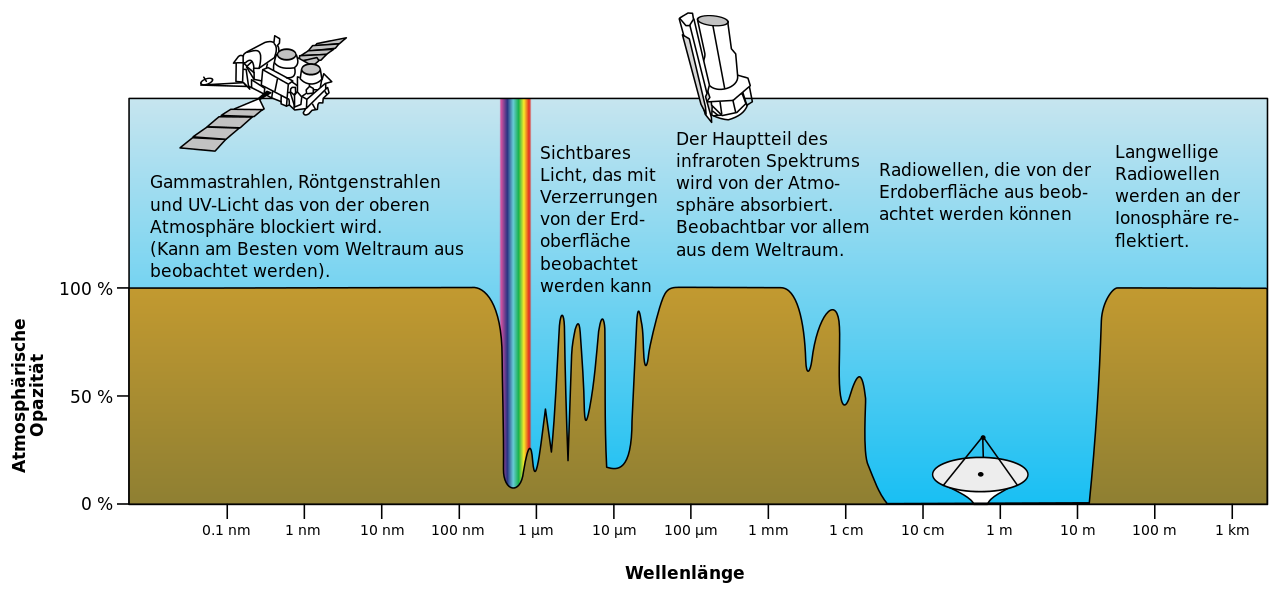
\includegraphics[width=0.99\textwidth]{./Plots/02_Astroteilchenphysik/Atmospheric_electromagnetic_opacity.png}
%     \caption{Zu sehen ist die Durchlässigkeit der Atmosphäre für elektromagnetische Strahlung in Abhängigkeit von der Wellenlänge.\cite{Opazitaet}}
%     \label{EM-Opazitaet}
% \end{figure}
% 
% 
% Wie in \autoref{EM-Opazitaet} zeigt, ist die Atmosphäre transparent für optische Beobachtungen und Radiowellen. 
% Alle anderen Wellenlängen werden von der Atmosphäre geblockt, sodass bis 1960 nur in diesen Wellenlängen beobachtet wurde.
% Mit der Entwicklung der Raumfahrt konnten dann auch Satellitenexperimente konzipiert werden, mit denen Gammaastronomie betrieben wurde.
% Aber auch mit bodengebundenen Experimenten wird Gammaastronomie betrieben mit Hilfe von Sekundärprodukten, die mit der Atmosphäre wechselwirken.
% Die minimale Energie, bei der Gammastrahlung auf der Erde detektiert werden kann ist zufällig genau über der maximalen Energie, die von Satellitenexperimenten beobachtet wird.
% Die bodenegebundenen Experimente beruhen auf der Detektion des Cherenkovlichts von elektromagnetischen Schauern in der Atmosphäre.\cite{Weekes}
% 
% Die bevorzugte Wechselwirkung eines Gammateilchen, das mit einer Energie $E>\SI{10}{MeV}$ in die Atmosphäre eintritt, ist die Paaarproduktion, die meist nach einer durchlaufenen Strecke von ca. $\SI{20}{km}$ auftritt.
% Das produzierte $e^+/e^-$-Paar fliegt in die gleiche Richtung wie das primäre Photon und wechselwirkt mit den Molekülen der Atmosphäre.
% Dabei werden Bremsstrahlungsphotonen emittiert, die dann eine weitere Paarproduktion auslösen können.
% Die resultierende Kaskade ist relativ schmal und bewegt sich in die gleiche Richtung wie das Ursprungsteilchen.
% Sie wächst so lange bis die Energie der geladenen Teilchen so gering ist, dass Ionisationsverluste und Strahlungsverluste gleich groß sind und erreicht da ihr Schauermaximum.
% Danach nimmt die Anzahl der Teilchen der Kaskade ab und der Schauer stirbt aus, was meistens über dem Erdboden passiert.
% Die sekundären geladenen Teilchen im Schauer emittieren Cherenkovlicht in Vorwärtsrichtung unter einem Winkel von ca. 1,3°, welches dann von den Teleskopen detektiert wird.
% Nicht nur primäre Photonen können solch einen Schauer induzieren, sondern auch Hadronen, wobei der Schauer kein rein elektromagnetischer ist. 
% Ein hadronischer Schauer unterscheidet sich in seiner Form von einem elektromagnetischen (siehe \todo{CORSIKA-Referenz}).\cite{Weekes}
% 
% Für die Detektion wird ein Detektor mit schneller Elektronik benötigt, mit dem Ziel den Ursprung des Schauers, die Energie und die Ankunftszeit zu bestimmen.
% Die Photonenanzahl im Schauer ist ein gutes Maß für die Energie des ursprünglichen Photons.
% Für eine große Sensitivität muss die Lichtsammelfläche eines Telskops möglichst groß sein. 
% Die Entwicklung von Teleskopen mit segmentierten Spiegeln begann mit dem Whipple-Teleskop\cite{Whipple}.
% Heute nutzen sowohl MAGIC\cite{MAGIC_Telescopes}, als auch HESS\cite{HESS} und VERITAS\cite{VERITAS} diese Technologie.
% Mit Hilfe von Photomultipliern (PMTs) wird eine hohe Sensitivität für blaue Wellenlängen bereitgestellt. 
% Problematisch ist, dass diese PMTs bei zu hellen Bedingungen nicht betrieben werden können und so eine Observation bei Vollmond nicht möglich ist.\cite{Weekes}
% 
% Für einen guten Standort muss auch das Störlicht minimiert werden. 
% Dies kann durch eine geschickte Standortwahl z.B. auf hohen Bergen fernab von Städten gewährleistet werden.

Wie in \ref{subsec:Photonen} beschrieben wurde, lässt sich die Gammaastronomie in verschiedene Energiebereiche einteilen.
Abhängig vom Energiebereich werden verschiedene Detektoren benötigt.

\paragraph{Satellitenexperimente}
Gammastrahlung mit Energien, die kleiner sind als $\SI{10}{GeV}$ werden mit Satellitenexperimenten detektiert.
Der Transport ins All stellt limitierende Bedingungen an diese Experimente.
Die Detektionsfläche ist relativ klein und aufgrund des kleinen Teilchenflusses werden lange Beobachtungszeiten benötigt.
Im Allgemeinen lassen sich abhängig vom dominanten Wechselwirkungsprozess in dem zu beobachtenden Energiebereich zwei Detektionstechniken unterscheiden.
Hochenergetische Gammastrahlung wird über den Prozess der Paarproduktion detektiert und die mittelenergetische Gammastrahlung über den Prozess der Comptonstreuung.\cite{Weekes}

Die Paarproduktionsteleskope arbeiten typischerweise im Energiebereich von ca. $\SI{30}{MeV}$-$\SI{10}{GeV}$.
Die Experimente COS-B \cite{CosB} und EGRET \cite{EGRET} sind zwei Beispiele für diesen Typ.
Sie nutzen Funkenkammern zur Detektion der Sekundärteilchen und bestehen aus verschiedenen Bauteilen.
EGRET \cite{EGRET} an Bord des \textit{CGRO} besteht aus einem Tracker, der eine Funkenkammer beinhaltet.
Ein Gammastrahlungsphoton erzeugt innerhalb dieses Trackers ein Elektron-Positron-Paar, welches in der Funkenkammer detektiert wird.
Der Pfad dieses Paars wird in der Kammer aufgezeichnet.
Jedes Elektron-Positron-Paar, welches die Funkenkammer verlässt, wird dann vom sogenannten Trigger gezählt.
Mit Hilfe des dritten Bauteils, dem Kalorimeter, wird die Energie des Paars bestimmt.
Als Veto dient eine Umhüllung des Detektors, die geladene Teilchen detektiert, die nicht innerhalb des Detektors erzeugt werden.\cite{Weekes}

Comptonteleskope dienen der Detektion von Gammastrahlung im Energiebereich $\SI{100}{keV}$-$\SI{10}{MeV}$.
Sie bestehen aus einem Szintillationsdetektor aus festem oder flüssigen Material, in dem Licht von geladenen Sekundärteilchen detektiert wird.
Diese Sekundärteilchen sind in einer Comptonstreuung mit Gammastrahlung entstanden.
Mit Hilfe von Photomultipliern (PMTs) wird das Licht detektiert.
Auch diese Teleskope sind von einer Veto-Umhüllung umgeben.\cite{Weekes}

\paragraph{Erdgebundene Gammaastronomie}
Die erdgebundenen Experimente beruhen auf der Entwicklung einer elektromagnetischen Kaskade in der Atmosphäre.
Trifft ein Photon mit einer Energie, die größer als $\SI{10}{MeV}$ ist, auf die Atmosphäre, dann produziert es typischerweise in einer Höhe von ca. $\SI{20}{km}$ ein Elektron-Positron-Paar.
Diese Paarproduktion erfolgt in Vorwärtsrichtung.
In dem typischen Energiebereich für erdgebundene Gammaaastronomie $E>\SI{10}{GeV}$ wechselwirkt dieses Paar mit den Molekülen der Luft.
Dabei entstehen in Bremsstrahlungsprozessen Photonen, die wiederum weitere Paare produzieren.
So entsteht eine elektromagnetische Kaskade in der Atmosphäre.
Diese Kaskade wächst so lange bis Ionisations- und Strahlungsverluste gleich groß sind und das Schauermaximum erreicht ist.
Danach stirbt der Schauer langsam aus.
Begleitet wird der Schauer von Cherenkovphotonen.
Diese entstehen sobald die Energie der Sekundärelektronen oberhalb der Schwelle für Cherenkovemission liegt.
Photonen werden in Vorwärtsrichtung unter dem sogenannten Cherenkovwinkel emittiert. 
Dieser Winkel beträgt auf Meereshöhe ca. $1.3°$.\cite{Weekes}

Nur ein kleiner Teil Primärteilchenenergie ($<10^{-6}$) geht in die Emission des sichtbaren Cherenkovlichts.
Allerdings ist dieses Licht mit Hilfe eines Spiegels und PMTs einfach zu detektieren.
Weiterhin ist es möglich aus dem Cherenkovlicht Rückschlüsse auf den Ursprung, die Energie, sowie die Ankunftszeit des Primärteilchens zu ziehen.
Bei den für Cherenkovteleskope interessanten Energien ($E\gtrsim \SI{100}{GeV}$) verhält sich die Atmosphäre wie ein großes Kalorimeter und die Helligkeit des Cherenkovlichtkegels am Boden bietet ein gutes Maß für die Primärteilchenenergie.
Das Cherenkovlicht kommt innerhalb einiger Nanosekunden am Detektor an.
Bei einem Schauer, der von einem Primärteilchen mit der Energie $E=\SI{1}{TeV}$ ausgelöst wurde, kommen 25\% des Lichts von Schauerteilchen in Höhe der ersten Wechselwirkung.
Der Hauptanteil (ca. $50\%$) wird von einem Zylinder der Länge $\SI{4}{km}$ im Schauermaximum emittiert.
Dieses Licht stellt ein gutes Maß für die totale Energie des Schauers dar.
Die letzten $25\%$ werden von Schauerteilchen unterhalb von $\SI{6}{km}$ emittiert.\cite{Weekes}

Die Grundidee der atmosphärischen Cherenkovtechnik ist einfach.
Es wird ein Lichtdetektor benötigt, der sich in der Fokalebene eines Spiegels befindet, sowie schnelle Ausleseelektronik.
Schon mit solch einem einfachen Detektor mit einer Lichtsammelfläche von $\SI{2}{km^2}$ und einer Integrationszeit von $\SI{10}{ns}$ ist es möglich, ein Lichtsignal eines Schauers mit Primärteilchenergie $\SI{1}{TeV}$ zu detektieren.
Allerdings ist die Unterscheidung zwischen einem elektromagnetischen Schauer, ausgelöst von Gammastrahlung, und einem Schauer ausgelöst von kosmischer Strahlung schwierig.\cite{Weekes}

Die Ionen und Protonen der kosmischen Strahlung wechselwirken ebenfalls in der Atmosphäre und lösen hadronische Kaskaden aus, die den elektromagnetischen Kaskaden sehr ähnlich sind.
Auch Teilchen dieser hadronischen Schauer emittieren Cherenkovlicht, sodass Teleskope der ersten Generation diese Schauer nicht voneinander unterscheiden konnten.
Außerdem ist zu beachten, dass der hadronische Untergrund ca. $10^3$ mal so groß ist.
Von Vorteil ist, dass sich hadronische Schauer von elektromagnetischen in einigen Eigenschaften leicht unterscheiden.
So besitzen diese beiden Arten von Schaueren unterschiedliche laterale Verteilungen, zeitliche Verteilungen, eine anderes Lichtspektrum, sowie eine andere Winkelverteilung.\cite{Weekes}

Um einen Schauer detektieren zu können, sind einige Eigenschaften des Detektors bzw. der Umgebung von großer Bedeutung.
Die Atmosphäre spielt eine grundlegende Rolle, stellt den Beobachter aber vor Herausforderungen. 
Aufgrund von Wolken ist die Transmission variabel, sodass die Bewölkung, sowie das Wetter überwacht werden müssen.
Das Mond- und Sternenlicht, sowie Menschen-gemachte Lichtquellen sollten ebenfalls minimiert werden, um gute Beobachtungsbedingungen zu erreichen. 
Das geschieht durch eine gute Standortwahl.
Detektor-spezifische Eigenschaften wie eine möglichst große Lichtsammelfläche werden durch segmentierte Spiegel erreicht und Lichtdetektoren, die sensitiv für Cherenkovlicht sind, werden in Form von PMTs bereitgestellt.\cite{Weekes}

Wird eine größere Anzahl an PMTs in der fokalen Ebene eines großen Reflektors angeordnet, stellen diese eine Kamera dar.
Die Cherenkovphotonen des Schauers, die am Spiegel reflektiert werden, erzeugen dann in der Kamera ein Bild, welches parametrisiert und analysiert werden kann.
Anhand der Bildparameter und anhand der Orientierung zum Kamerazentrum ist es mit dieser Technik möglich, elektromagnetische Schauer von hadronischen zu unterscheiden.
Diese Technik wird Imaging Air Cherenkov (IACT)-Technik genannt und von vielen großen Teleskopen bzw. Teleskoparrays wie den in dieser Arbeit betrachteten MAGIC-Teleskopen \cite{MAGIC_Telescopes}, aber auch HESS \cite{HESS}, VERITAS \cite{VERITAS} benutzt.\cite{Weekes}

Im Gegensatz zur IACT-Technik existieren noch andere bodengebundene Teleskope, die Gammaastronomie betreiben.
Erreicht ein Primärteilchen Energien, die größer sind als $\SI{10}{TeV}$, erreichen genug Teilchen des Schauers den Boden, sodass der Schauer direkt detektiert und Energie sowie Ankunftszeit rekonstruiert werden können.
Für diese Technik werden viele Teilchendetektoren auf einer großen Fläche verteilt.
Außerdem bietet diese Art der Detektion den Vorteil, dass eine durchgängige Observation möglich ist.
Als Beispiel dienen der MILAGRO-Detektor \cite{MILAGRO} in New Mexico, USA, sowie sein Nachfolgeexperiment HAWC \cite{HAWC}.
MILAGRO bestand aus ca. 700 Lichtdetektoren in einem See und ca. 200, die außen herum platziert wurden.
Auch das Pierre-Auger-Experiment \cite{AUGER}, welches sich in der südamerikanischen Pampa befindet ist ein gutes Beispiel.
Dieses Experiment beinhaltet ca. 1600 Oberflächendetektoren, die sich in Wassertanks befinden und 27 Fluoreszenzteleskope.
Mit diesen beiden Teleskoparten können die Eigenschaften der detektierten Schauer genau bestimmt werden.



\section{Aktive galaktische Kerne}
\label{sec:AGN}

\begin{figure}
    \centering
    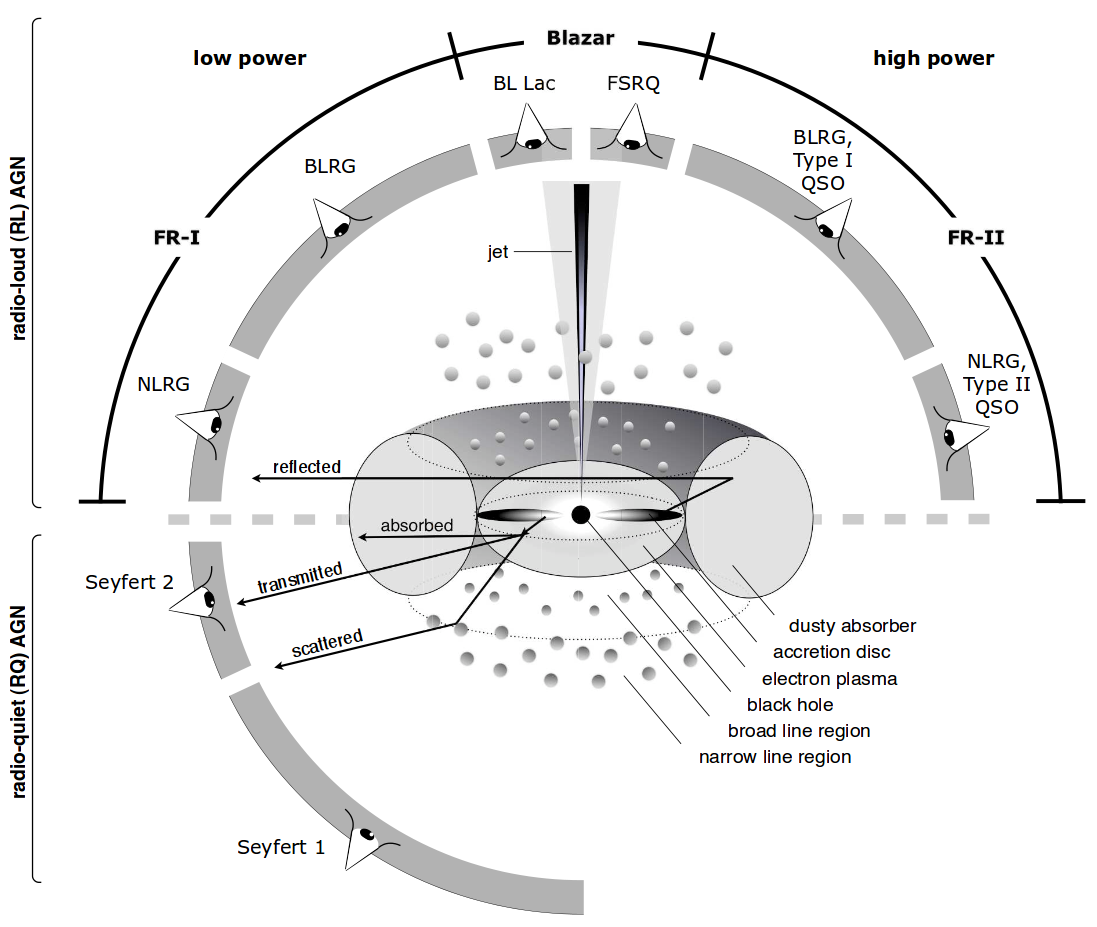
\includegraphics[width=0.8\textwidth]{./Plots/02_Astroteilchenphysik/AGN_Schema.png}
    \caption{Schema zur Klassifikation von AGN (siehe \autoref{subsec:Klassifikation}). Abhängig von der Radioemission und dem Blickwinkel werden die einzelnen AGN-Typen voneinander unterschieden.
    Im Inneren einer AGN befindet sich ein supermassives Schwarzes Loch, welches von einer Akkretionsscheibe umgeben ist. 
    Diese wird wiederum von einem Staubtorus umschlossen.
    Aus dem Zentrum werden zwei entgegengesetzte Jets emittiert.\cite{AGNSchema}}
    \label{AGN_Bild}
\end{figure}

% Wie in \autoref{AGN_Bild} zu sehen ist, befindet sich im Zentrum jeder AGN ein Supermassives Schwarzes Loch, welches Materie akkretiert und eine Akkretionsscheibe formt.
% Oberhalb der Scheibe befinden sich Wolken, die mit schneller Geschwindigkeit rotieren und Emissionslinien fabrizieren. Diese Region wird Broad Line Region (BLR) genannt.
% Wolken die mit einem größeren Abstand um das schwarze Loch kreisen produzieren die narrow lines und werden Narrow Line Region genannt.
% Die BLR und die zentrale Region sind von einem Staubtorus umgeben.
% Senkrecht zur Scheibe werden zwei Jets in entgegengesetzte Richtungen emittiert.\cite{Weekes}

Aktive galaktische Keren produzieren sehr hohe Luminositäten in einem sehr konzentrierten Volumen.
Die Prozesse, die dazu führen, sind vermutlich andere Prozesse als die Kernfusion in ``normalen Sternen''.
Wie in \autoref{AGN_Bild} zu sehen ist, befindet sich im Zentrum einer AGN ein supermassives Schwarzes Loch, welches von einer Akkretionsscheibe umgeben ist.
Die Materie dieser Scheibe wird vom Schwarzen Loch akkretiert und verliert dabei Drehimpuls.
Von der Akkretionsscheibe wird UV-Licht und manchmal auch schwache Röntgenstrahlung emittiert.
Auch harte Röntgenstrahlung wird sehr nahe am Schwarzen Loch produziert.
Durch die Rotation kann das Schwarze Loch Energie emittieren.
Umhüllt sind das zentrale Schwarze Loch und die Akkretionsscheibe von einem Staubtorus.
Im Potential des Schwarzen Lochs befinden sich Gaswolken, die sich schnell bewegen und dabei starke optische und ultraviolette Emissionslinien produzieren, die abhängig von der Sichtlinie und der Lage des Staubtorusses beobachtet werden können. 
Diese Wolken werden ``Broad Line Clouds'' genannt.
Außerhalb des Torus sind Gaswolken, die sich langsamer bewegen und schmale Emissionslinien produzieren.
Eine Emission von energiereichen Teilchen erfolgt in Form zweier Jets, die in entgegengesetzten Richtungen emittiert werden.
In diesen Jets strömt das Plasma mit hohen Geschwindigkeiten und strahlt relativistisch in Vorwärtsrichtung.
Die Achsensymmetrie dieses Modells impliziert, dass AGNs abhängig von der Lage zum Beobachter unterschiedlich aussehen und sich unterschiedlich verhalten.
Anhand dieser Eigenschaften können AGNs klassifiziert werden (siehe \autoref{subsec:Klassifikation}).
In der Erforschung von AGNs sind fundamentale Eigenschaften wie die Masse des Schwarzen Lochs oder aber der Spin von Bedeutung.
Mit Hilfe dieser Eigenschaften können eventuell die Materieakkretion oder die Jetbildung verstanden werden.\cite{Urry_Padovani}


\subsection{Klassifikation}
\label{subsec:Klassifikation}
% Nach Urry und Padovani\cite{Urry_Padovani} werden AGNs in radiolaute und radioleise Vertreter unterteilt. 
% Diese werden dann wieder gemäß ihrer Ausrichtung zur Sichtlinie des Beobachters weiter klassifiziert.
% Für eine genauere Informationen siehe \cite{Urry_Padovani}.
% Gemäß dieser Klassifikation werden nun Blazare betrachtet.
% Bei diesem AGN-Typ handelt es sich um radiolaute Quellen und der Beobachter guckt in den Jet. 
% Blazare können in allen Wellenlängen beobachtet werden, d.h. über die volle Breite des elektromagnetischen Spektrums, was ca. 19 Dekaden in der Energie entspricht.
% Sie zeichnen sich durch ihre hohe Luminosität im Gammawellenlängenbereich und große Variabilität in allen Wellenlängen aus.
% Des Weiteren können starke Korrelationen zwischen den Wellenlängen beobachtet werden.\cite{Weekes}
Der Quelltyp der AGN umfasst einen Zoo an unterschiedlichen Subtypen mit verschiedenen Namen und Eigenschaften.
Wie \autoref{AGN_Bild} zeigt, werden nach Urry und Padovani \cite{Urry_Padovani} AGNs in radiolaute, AGNs mit Radioemission, und radioleise Vertreter, AGNs ohne Radioemission, unterteilt.
Des Weiteren erfolgt eine Unterscheidung in Typ I mit breiten Emissionslinien und Typ II mit schmalen Emissionslinien.
Innerhalb dieser Gruppen erfolgt eine weitere Unterteilung anhand der Luminosität.
Insgesamt sind ca. 15-20\% \cite{Urry_Padovani} der AGN radiolaut.
Mit wenigen Ausnahmen sind die Spektren im optischen und ultravioletten, sowie im Infraroten bis zu weicher Röntgenstrahlung bei allen AGNs ähnlich.
Die Radioemission hängt vermutlich zusammen mit dem Host-Galaxie-Typ oder dem Spin des Schwarzen Lochs, womit die Produktion von Jets erklärt werden kann.
Basierend auf den optischen und ultravioletten Emissionslinien können AGNs in drei Typen eingeteilt werden \cite{Urry_Padovani}:

\begin{itemize}
 \item Typ 1 beinhaltet AGNs mit breiten Emissionslinien, die von heißem Gas, welches sich mit hoher Geschwindigkeit bewegt, stammen.
 Die radioleisen Vertreter dieser Gruppe werden Seyfert 1 genannt und sind gekennzeichnet durch ihre geringe Luminosität, weswegen sie nur in kurzen Entfernungen detektiert werden können.
 Die radiolauten Vertreter werden zum einen Broad Line Radio Galaxy (BLRG) genannt und sind ebenfalls durch niedrige Luminosität gekennzeichnet. 
 Zum anderen gibt es die radiolauten Quasare mit hoher Luminosität, hier Quasi-stellar Object (QSO), genannt.
 \item Typ 2 beinhaltet die AGNs mit schmalen Emissionslinien, die von langsamem Gas emittiert werden, bzw. die Sichtlinie auf die Emission schneller Gasteilchen wird durch den Staubtorus blockiert.
 Die radioleisen Vertreter dieses Typs werden Seyfert 2 genannt und zeichnen sich duch geringe Luminosität aus.
 Die radiolauten AGNs werden Narrow Line Radio Galaxy (NLRG) bezeichnet und Fanaroff und Riley haben diese wiederum unterteilt in zwei Subtypen.
 Diese sind zu einen die Fanaroff \& Riley I (FR I), welche von geringer Luminosität geprägt sind und deren symmetrischen Radiojets in der Intensität nach außen hin abnehmen.
 Zum anderen gibt es noch den Fanaroff \& Riley II-Typ, dessen Jets gebündelt sind und in Radiolobes enden, in denen heiße Dichteschwankungen, genannt Hot Spots, sind.
 \item Der Typ 0 wird im Allgemeinen als Blazar bezeichnet und ist charakterisiert durch den sehr kleinen Winkel zwischen Jet und Beobachter.
 Dieser Typ beinhaltet den Flat Spectrum Radio Quasar (FSRQ), der sehr variabel ist und breite Emissionslinien wie Typ I-Objekte besitzt.
 Außerdem gehören die BL-Lac-Objekte zu dieser Klasse. Diese haben keine starken Emissionslinien.
 Die analysierte Quelle Mrk~421 gehört zum Typ BL-Lac.
 BL-Lacs können in allen Wellenlängen beobachtet werden, d.h. über die volle Breite des elektromagnetischen Spektrums, was 19 Dekaden in der Energie entspricht.
 Sie zeichnen sich durch ihre hohe Luminosität im Gammawellenlängenbereich aus und besitzen eine hohe Variabilität in allen Wellenlängen.
 Außerdem konnten starke Korrelationen zwischen den Wellenlängen beobachtet werden.
\end{itemize}


\subsection{Spektrale Energieverteilung}
Eine spektrale Energieverteilung (SED: Spectral Energy Distribution) beschreibt die Emission einer Quelle in Abhängigkeit von den verschiedenen Wellenlängen.
Die SEDs von Blazaren besitzen eine charakteristische Struktur mit zwei Höckern.
Bei sehr hochenergetischen Blazaren, wie z.B. Mrk 421 und Mrk 501, befindet sich ein Peak bei Röntgenenergien und ein anderer Peak bei (10-250)$\si{GeV}$.
Beide Peaks sind vergleichbar hoch, was charakteristisch für diesen Quelltyp ist.\cite{Weekes}


\subsection{Variabilität}
Blazare besitzen charakteristische Variabilitäten zwischen einigen Minuten und Jahren.
Die erste Detektion eines Flares, also eines außergewöhnlichen Flussanstiegs, in der VHE-Emission einer AGN fand 1994 statt:
Whipple beobachtete einen Flussanstieg von Mrk~421 auf den zehnfachen Wert.\cite{Weekes}\cite{Mrk421_Outburst}

\subsection{Multiwellenlängenbeobachtungen}
Die simultane Beobachtung einer Quelle mit mehreren Teleskopen zur genauen Aufnahme der Aktivität in allen Wellenlängen wird Multiwellenlängenbeobachtung (MWL-Beobachtung) genannt. 
Diese Beobachtungen dienen u.a. dazu, Rückschlüssen auf die Beschleunigungsmechanismen in den Quellen zu ziehen.
Es können Korrelationen der Flüsse in verschiedenen Wellenlängen untersucht werden.
Die erste MWL-Kampagne wurde 1995 organisiert; Ziel war die Quelle Mrk~421.\cite{Weekes}

\subsection{Modelle für hochenergetische Gammaemission}
Es existieren grundsätzlich zwei verschiedene Ansätze um die hochenergetische Gammaemission zu erklären.
Dies sind zum einen leptonische Modelle und zum anderen hadronische Modelle.
Im Folgenden werden zuerst zwei mögliche leptonische Modelle und anschließend ein hadronisches Modell vorgestellt.

\subsubsection{Leptonische Modelle}
Die spektrale Energieverteilung (SED) gibt Hinweise auf die Strahlungsmechanismen, die sich im Inneren eines Jets ereignen können.
Im Inneren eines Jets werden Elektronen durch Schocks beschleunigt. 
Diese Schocks entstehen durch Materieansammlungen, die den Jet mit verschiedenen Geschwindigkeiten durchlaufen.
Die beschleunigten Elektronen verlieren ihre Energie durch Synchrotronstrahlung im Magnetfeld des Jets und produzieren den Synchrotronpeak in der SED.
Die Position dieses Peaks wird durch die Effizienz der Schockbeschleunigung und der Cooling-Prozesse, d.h. der Energieverluste bestimmt. 
Im Folgenden werden zwei verschiedene leptonische Modelle vorgestellt.\cite{Weekes}

\begin{itemize}
\item Im Synchrotron-Selbst-Compton-Modell (SSC-Modell) werden die in Synchrotron-Prozessen abgestrahlten Photonen zu hohen Energien beschleunigt, die nahe an den Elektronenergien sind.
Im Thomson-Regime können Photonenergien von $E_{\gamma}\approx \gamma^2 h \nu$ und im Klein-Nishina-Regime $E_{\gamma}\approx \gamma m_e c^2$ erreicht werden.\cite{Weekes}
\item Im External-Radiation-Compton-Modell (ERC-Modell) werden sogenannte Saat-Photonen benötigt, die dann eine inverse Comptonstreuung erfahren.
Diese Saat-Photonen werden außerhalb des Jets produziert, z.B. in der Akkretionsscheibe.\cite{Weekes}
\end{itemize}

\subsubsection{Hadronische Modelle}
Als Beispiel für ein hadronisches Modell wird im Folgenden das Proton-Modell vorgestellt.
In dem Proton-Modell wird die Gammastrahlung in Proton-induzierten Kaskaden produziert. 
Ziel dieser Modelle ist es, zwei Phänome gleichzeitig zu erklären: 
Dies sind zum einen die Produktion von VHE-Gammastrahlung in AGNs und zum anderen der Ursprung der extragalaktischen kosmischen Strahlung mit Energien von bis zu $10^{20}\,\si{eV}$.
Die sehr hochenergetische Gammastrahlung entsteht durch beschleunigte Protonen im Jet mit Energien von bis zu $10^{18}\,\si{eV}$, die dann mit niederenergetischeren Photonen wechselwirken und Pionen produzieren.
Die erzeugten Pionen zerfallen und lösen eine Kaskade aus.
In manchen Modellen wird die Gammastrahlung als Synchrotronstrahlung von sehr energiereichen Protonen emittiert.
Das Problem der Proton-Modelle ist, dass kurze Zeitvariabilitäten nicht erklärt werden können, da dafür ein sehr schnelles Cooling der Protonen nötig wäre. 
Durch Synchrotronstrahlung können die Protonen nicht schnell genug abgebremst werden.
Kollisionen mit Photonen oder Ionen im Jet wären eine bessere Erklärung.
In jedem Fall können hadronische Modell erst dann verifiziert werden, wenn ein Neutrinofluss, resultierend aus dem Pion-Zerfall detektiert wird.\cite{Weekes}


\section{Markarian 421}
\label{sec:Mrk421}

Die AGN Markarian 421 (Mrk 421) (RA=$11^h 4^m 27,31^s$, Dec=$38°12' 31,8''$) wurde 1992 von Whipple als Gammastrahlungsquelle entdeckt \cite{EntdeckungWhipple}.
Sie ist eine der hellsten extragalaktischen Quellen im Röntgen- und TeV-Licht und wird dem Typ BL-Lac zugeordnet.
Sie besitzt eine Rotverschiebung von $z=0,0031$ und ist damit die von uns nächste extragalaktische Quelle im TeV-Energiebereich.\cite{MWL2009}

\begin{figure}
    \centering
    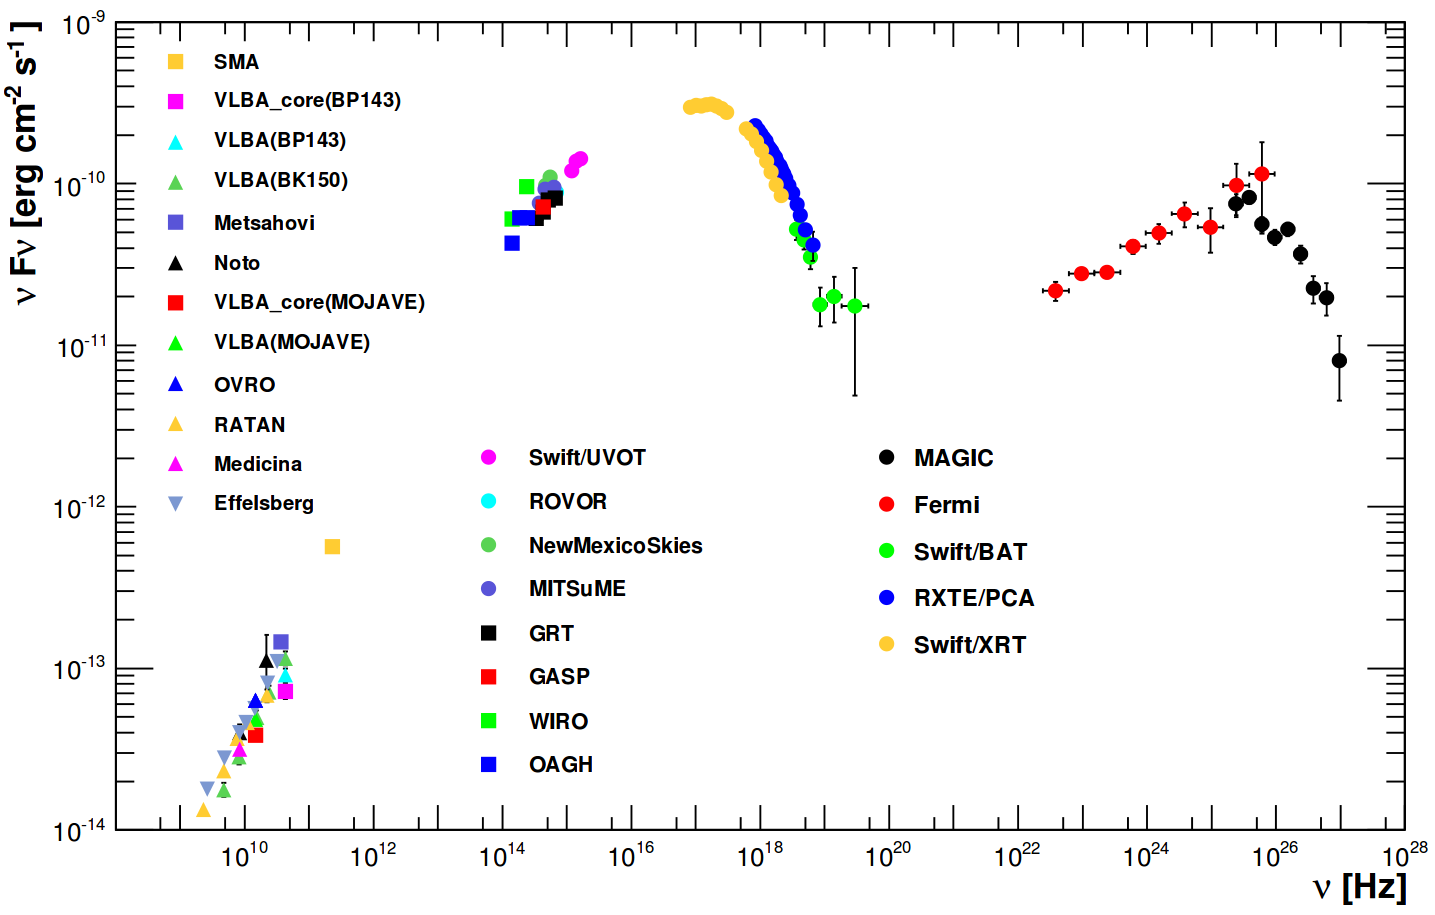
\includegraphics[width=0.9\textwidth]{./Plots/02_Astroteilchenphysik/SED_Mrk421.png}
    \caption{Die Abbildung zeigt die spektrale Energieverteilung von Mrk 421. Die für Blazare typische doppelhöckrige Struktur ist erkennbar. 
     Des Weiteren ist zu sehen, dass das Maximum des niederenergetischen und des hochenergetischen Höckers einen ähnlichen Fluss aufweist.\cite{Mrk421_SED}}
    \label{Mrk_SED}
\end{figure}

\autoref{Mrk_SED} zeigt die spektrale Energieverteilung von Mrk~421, mit Daten einer MWL-Kampagne zwischen dem 19.1.2009 und dem 1.6.2009. 
Es wurde der Energiebereich von Radiowellen bis sehr hochenergetischer Gammastrahlung einbezogen.
Die für BL-Lacs charakteristische doppelhöckrige Struktur ist zu sehen mit Peaks bei keV-Energien und bei GeV-TeV-Energien.
Die SED kann mit Hilfe von SSC-Modellen beschrieben werden, allerdings sind hadronische Modelle trotzdem nicht auszuschließen.

\begin{figure}
    \centering
    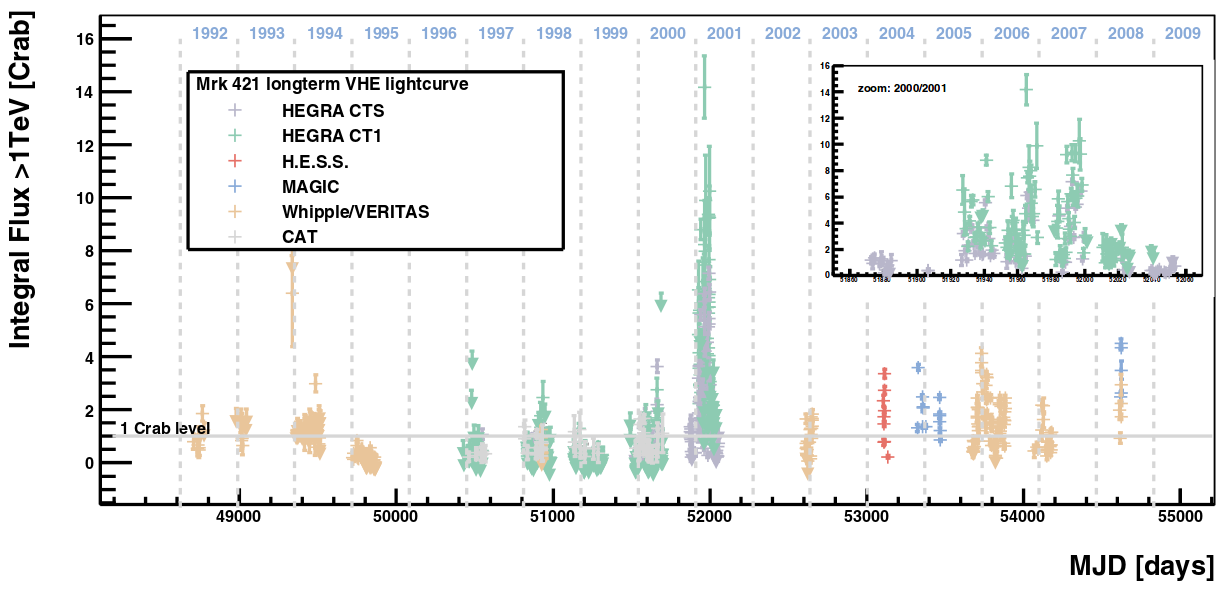
\includegraphics[width=0.9\textwidth]{./Plots/02_Astroteilchenphysik/Mrk421_LC_lang.png}
    \caption{Die Abbildung zeigt eine Lichtkurve von Mrk~421, die zwischen 1992 und 2009 aufgenommen wurde.
    Die Variabilität dieser Quelle ist deutlich zu erkennen, wobei 2001 die größte Aktivität herrschte.\cite{Mrk421_LC_lang}}
    \label{Mrk421_LC_Alles}
\end{figure}

\autoref{Mrk421_LC_Alles} zeigt eine Lichtkurve von Mrk~421, die zwischen 1992 und 2009 aufgenommen wurde.
Deutlich sind die Unterschiede zwischen Zeiten niedriger und hoher Aktivität zu erkennen. 
Das Jahr 2001 ist geprägt von hoher Aktivität und der Fluss liegt zwischendurch bei mehr als dem zehnfachen Fluss von Crab.\cite{Mrk421_LC_lang}
Die Kurzzeitvariabilität dieser Quelle ist ebenfalls so ausgeprägt, dass eine Verdopplung des Flusses in $\SI{15}{min}$ beobachtet werden konnte.\cite{Weekes}

Mit Hilfe von MWL-Kampagnen konnten sowohl während aktiver als auch während nicht aktiver Zeiten Korrelationen zwischen der Röntgen- und Gammastrahlungsemission gefunden werden.
Aus diesen Multiwellenlängenbeobachtungen wird geschlossen, dass mit Hilfe eines leptonischen Modells die Emission der Quelle gut beschrieben werden kann.\cite{MWL2009}


% 
% 
% Die Quelle ist sehr variabel; so wurde z.B. schon eine Verdopplung des Flusses in $\SI{15}{min}$ beobachtet.
% %Es wurden Variationen im Fluss von mehr als einer Ordnung in der Magnitude beobachtet und eine Verdopplung des Flusses in 15min.
% Während eines Flares konnte auch eine Änderung in der Steigung des Spektrums beobachtet werden.
% In MWL-Kampagnen wurden auch Korrelationen von verschiedenen Wellenlängen beobachtet.
% Die charakteristische doppelhöckrige Struktur in der SED ist ebenfalls erkennbar, wobei der erste Peak bei keV-Energien und der zweite bei GeV-TeV-Energien zu erkennen ist (siehe \autoref{Mrk_SED}). 
% Mit Hilfe des SSC-Modells kann die Form der SED gut beschrieben werden, wobei hadronische Modelle trotzdem nicht auszuschließen sind.
% Die ersten Beobachtungen von MAGIC im Winter 2004/2005 und im Frühling 2005 beinhalten Observationen von Mrk 421.
% Eine Multiwellenlängenkampagne von der Quelle hat auch, während die Quelle in einem nicht aktiven Zustand war, Variabilitäten beobachtet und eine Korrelation zwischen VHE und Röntgenstrahlung destgestellt \cite{MWL2009}.\cite{Weekes}